\documentclass{standalone}
\usepackage{tikz}
\usetikzlibrary{patterns, positioning}


\begin{document}
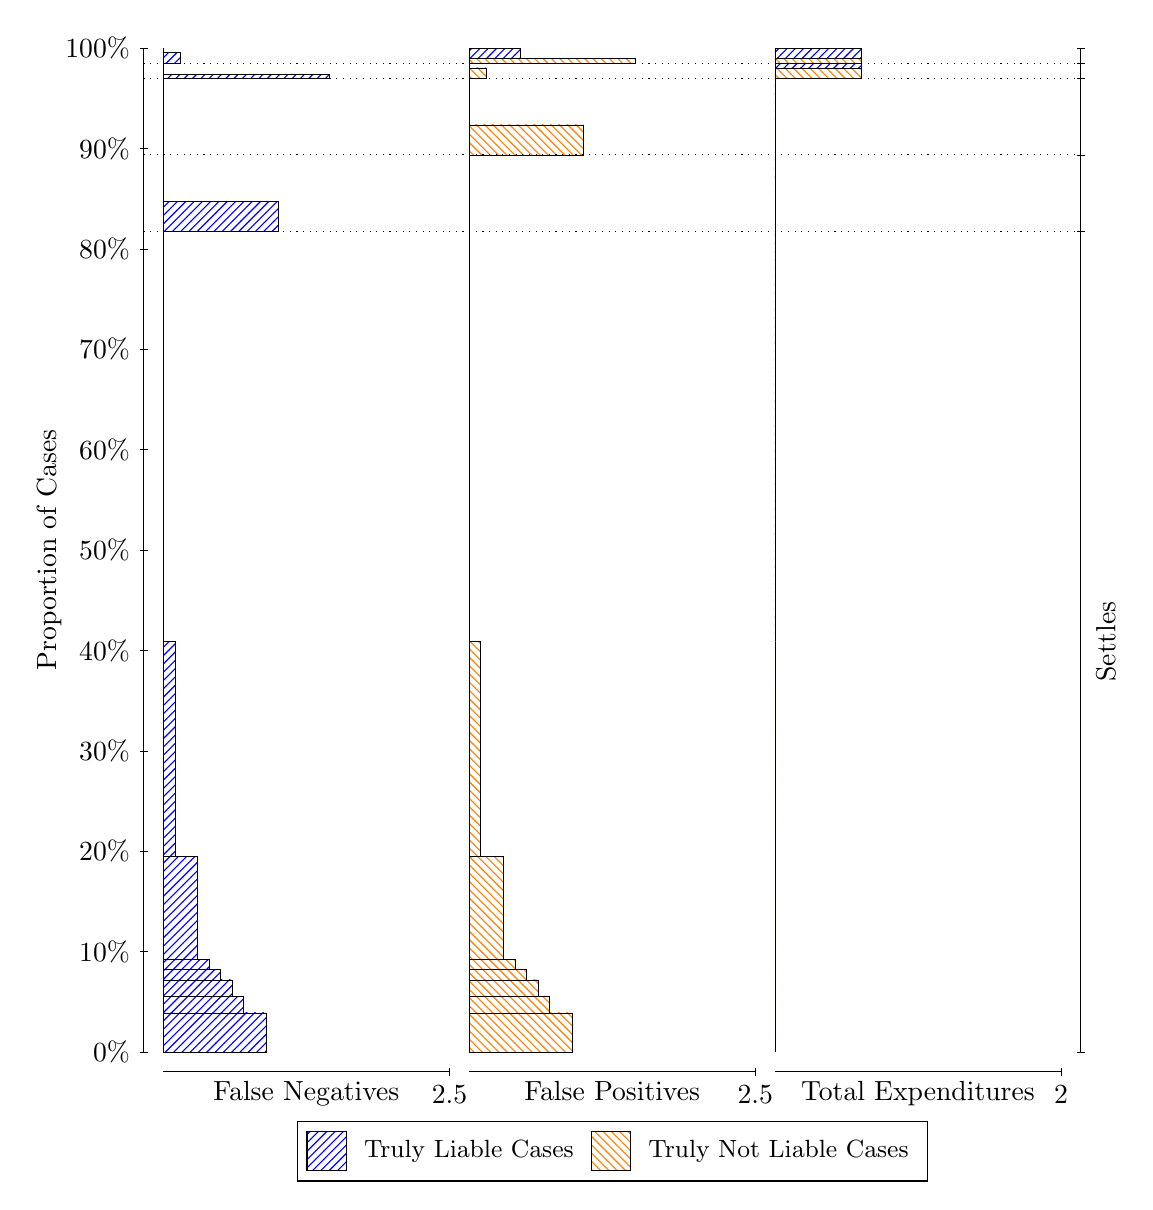
\begin{tikzpicture}
\draw[black, very thin] (1.5,1.75) -- (1.5,14.5);
\node[rotate=90, text=black, anchor=center] at (0.3, 8.125) {Proportion of Cases};
\draw[black, very thin] (1.45,1.75) -- (1.55,1.75);
\node[text=black, anchor=east] at (1.45, 1.75) {0\%};
\draw[black, very thin] (1.45,3.025) -- (1.55,3.025);
\node[text=black, anchor=east] at (1.45, 3.025) {10\%};
\draw[black, very thin] (1.45,4.3) -- (1.55,4.3);
\node[text=black, anchor=east] at (1.45, 4.3) {20\%};
\draw[black, very thin] (1.45,5.575) -- (1.55,5.575);
\node[text=black, anchor=east] at (1.45, 5.575) {30\%};
\draw[black, very thin] (1.45,6.85) -- (1.55,6.85);
\node[text=black, anchor=east] at (1.45, 6.85) {40\%};
\draw[black, very thin] (1.45,8.125) -- (1.55,8.125);
\node[text=black, anchor=east] at (1.45, 8.125) {50\%};
\draw[black, very thin] (1.45,9.4) -- (1.55,9.4);
\node[text=black, anchor=east] at (1.45, 9.4) {60\%};
\draw[black, very thin] (1.45,10.675) -- (1.55,10.675);
\node[text=black, anchor=east] at (1.45, 10.675) {70\%};
\draw[black, very thin] (1.45,11.95) -- (1.55,11.95);
\node[text=black, anchor=east] at (1.45, 11.95) {80\%};
\draw[black, very thin] (1.45,13.225) -- (1.55,13.225);
\node[text=black, anchor=east] at (1.45, 13.225) {90\%};
\draw[black, very thin] (1.45,14.5) -- (1.55,14.5);
\node[text=black, anchor=east] at (1.45, 14.5) {100\%};

\draw[black, very thin] (13.4,1.75) -- (13.4,14.5);
\draw[black, very thin] (13.35,1.75) -- (13.45,1.75);
\node[anchor=west] at (13.35, 1.75) {};
\draw[black, very thin] (13.35,12.175) -- (13.45,12.175);
\node[anchor=west] at (13.35, 12.175) {};
\draw[black, very thin] (13.35,13.144) -- (13.45,13.144);
\node[anchor=west] at (13.35, 13.144) {};
\draw[black, very thin] (13.35,14.112) -- (13.45,14.112);
\node[anchor=west] at (13.35, 14.112) {};
\draw[black, very thin] (13.35,14.306) -- (13.45,14.306);
\node[anchor=west] at (13.35, 14.306) {};
\draw[black, very thin] (13.35,14.5) -- (13.45,14.5);
\node[anchor=west] at (13.35, 14.5) {};

\draw[black, very thin, pattern color=blue, pattern=north east lines] (1.75,1.75) rectangle (3.058,2.2457);
\draw[black, very thin, pattern color=blue, pattern=north east lines] (1.75,2.2457) rectangle (2.7673,2.4514);
\draw[black, very thin, pattern color=blue, pattern=north east lines] (1.75,2.4514) rectangle (2.622,2.6657);
\draw[black, very thin, pattern color=blue, pattern=north east lines] (1.75,2.6657) rectangle (2.4767,2.803);
\draw[black, very thin, pattern color=blue, pattern=north east lines] (1.75,2.803) rectangle (2.3313,2.9299);
\draw[black, very thin, pattern color=blue, pattern=north east lines] (1.75,2.9299) rectangle (2.186,4.2346);
\draw[black, very thin, pattern color=blue, pattern=north east lines] (1.75,4.2346) rectangle (1.8953,6.9625);
\draw[black, very thin, pattern color=orange, pattern=north west lines] (1.75,6.9625) rectangle (1.75,12.175);
\draw[black, very thin, pattern color=blue, pattern=north east lines] (1.75,12.175) rectangle (3.2033,12.556);
\draw[black, very thin, pattern color=orange, pattern=north west lines] (1.75,12.556) rectangle (1.75,13.144);
\draw[black, very thin, pattern color=orange, pattern=north west lines] (1.75,13.144) rectangle (1.75,13.524);
\draw[black, very thin, pattern color=blue, pattern=north east lines] (1.75,13.524) rectangle (1.75,14.112);
\draw[black, very thin, pattern color=blue, pattern=north east lines] (1.75,14.112) rectangle (3.8573,14.17);
\draw[black, very thin, pattern color=orange, pattern=north west lines] (1.75,14.17) rectangle (1.75,14.306);
\draw[black, very thin, pattern color=blue, pattern=north east lines] (1.75,14.306) rectangle (1.968,14.442);
\draw[black, very thin, pattern color=orange, pattern=north west lines] (1.75,14.442) rectangle (1.75,14.5);
\draw[black, very thin, pattern color=orange, pattern=north west lines] (5.6333,1.75) rectangle (6.9413,2.2457);
\draw[black, very thin, pattern color=orange, pattern=north west lines] (5.6333,2.2457) rectangle (6.6507,2.4513);
\draw[black, very thin, pattern color=orange, pattern=north west lines] (5.6333,2.4513) rectangle (6.5053,2.6656);
\draw[black, very thin, pattern color=orange, pattern=north west lines] (5.6333,2.6656) rectangle (6.36,2.8029);
\draw[black, very thin, pattern color=orange, pattern=north west lines] (5.6333,2.8029) rectangle (6.2147,2.9298);
\draw[black, very thin, pattern color=orange, pattern=north west lines] (5.6333,2.9298) rectangle (6.0693,4.2347);
\draw[black, very thin, pattern color=orange, pattern=north west lines] (5.6333,4.2347) rectangle (5.7787,6.9627);
\draw[black, very thin, pattern color=blue, pattern=north east lines] (5.6333,6.9627) rectangle (5.6333,12.175);
\draw[black, very thin, pattern color=orange, pattern=north west lines] (5.6333,12.175) rectangle (5.6333,12.763);
\draw[black, very thin, pattern color=blue, pattern=north east lines] (5.6333,12.763) rectangle (5.6333,13.144);
\draw[black, very thin, pattern color=orange, pattern=north west lines] (5.6333,13.144) rectangle (7.0867,13.524);
\draw[black, very thin, pattern color=blue, pattern=north east lines] (5.6333,13.524) rectangle (5.6333,14.112);
\draw[black, very thin, pattern color=orange, pattern=north west lines] (5.6333,14.112) rectangle (5.8513,14.248);
\draw[black, very thin, pattern color=blue, pattern=north east lines] (5.6333,14.248) rectangle (5.6333,14.306);
\draw[black, very thin, pattern color=orange, pattern=north west lines] (5.6333,14.306) rectangle (7.7407,14.364);
\draw[black, very thin, pattern color=blue, pattern=north east lines] (5.6333,14.364) rectangle (6.2873,14.5);
\draw[black, very thin, pattern color=orange, pattern=north west lines] (9.5167,1.75) rectangle (9.5167,6.9627);
\draw[black, very thin, pattern color=blue, pattern=north east lines] (9.5167,6.9627) rectangle (9.5167,12.175);
\draw[black, very thin, pattern color=orange, pattern=north west lines] (9.5167,12.175) rectangle (9.5167,12.763);
\draw[black, very thin, pattern color=blue, pattern=north east lines] (9.5167,12.763) rectangle (9.5167,13.144);
\draw[black, very thin, pattern color=orange, pattern=north west lines] (9.5167,13.144) rectangle (9.5167,13.524);
\draw[black, very thin, pattern color=blue, pattern=north east lines] (9.5167,13.524) rectangle (9.5167,14.112);
\draw[black, very thin, pattern color=orange, pattern=north west lines] (9.5167,14.112) rectangle (10.607,14.248);
\draw[black, very thin, pattern color=blue, pattern=north east lines] (9.5167,14.248) rectangle (10.607,14.306);
\draw[black, very thin, pattern color=orange, pattern=north west lines] (9.5167,14.306) rectangle (10.607,14.364);
\draw[black, very thin, pattern color=blue, pattern=north east lines] (9.5167,14.364) rectangle (10.607,14.5);
\draw[black, dotted] (1.5,12.175) -- (13.4,12.175);
\draw[black, dotted] (1.5,13.144) -- (13.4,13.144);
\draw[black, dotted] (1.5,14.112) -- (13.4,14.112);
\draw[black, dotted] (1.5,14.306) -- (13.4,14.306);
\draw[black, very thin] (1.75,1.5) -- (5.3833,1.5);
\node[text=black, anchor=north] at (3.5667, 1.5) {False Negatives};
\draw[black, very thin] (5.3833,1.45) -- (5.3833,1.55);
\node[text=black, anchor=north] at (5.3833, 1.45) {2.5};

\draw[black, very thin] (5.6333,1.5) -- (9.2667,1.5);
\node[text=black, anchor=north] at (7.45, 1.5) {False Positives};
\draw[black, very thin] (9.2667,1.45) -- (9.2667,1.55);
\node[text=black, anchor=north] at (9.2667, 1.45) {2.5};

\draw[black, very thin] (9.5167,1.5) -- (13.15,1.5);
\node[text=black, anchor=north] at (11.333, 1.5) {Total Expenditures};
\draw[black, very thin] (13.15,1.45) -- (13.15,1.55);
\node[text=black, anchor=north] at (13.15, 1.45) {2};

\node[text=black, centered, rotate=90] at (13.72, 6.9626) {Settles};





\draw (7.449999999999999,1.5) node[draw=none] (baseCoordinate) {};
\begin{scope}[align=center]
        \matrix[scale=0.5, draw=black, below=0.5cm of baseCoordinate, nodes={draw}, column sep=0.1cm]{
            \node[rectangle, draw, minimum width=0.5cm, minimum height=0.5cm, pattern color=blue, pattern=north east lines] {}; &
            \node[draw=none, font=\small, text=black] (B) {Truly Liable Cases}; &
            \node[rectangle, draw, minimum width=0.5cm, minimum height=0.5cm, pattern color=orange, pattern=north west lines] {}; &
            \node[draw=none, font=\small, text=black] (B) {Truly Not Liable Cases}; \\
            };
\end{scope}

\end{tikzpicture}
\end{document}